\chapter{Bewegungserkennung}\label{chapter:motion-detection}
In diesem Kapitel sollen die Ergebnisse aus Kapitel \ref{chapter:dataset}
verwendet werden, um eine Bewegungserkennung zu entwickeln. Genauer gesagt soll
auch hier ein Modell entworfen werden, um diese Bewegungen zu erkennen und
klassifizieren. Zudem soll ein Ausblick auf Techniken gegeben werden, um weitere
bewegungsabhängige Eigenschaften mithilfe von KNNs zu extrahieren. Zum Beispiel
ist beim Ausüben von sportlichen Aktivitäten neben der Art auch die Frage, ob
die Bewegung richtig ausgeführt wurde, interessant. Aber auch das Vorhersagen
von zukünftigen Bewegungen anhand kürzlich getätigten Posen kann für einige
Anwendungen hilfreich sein. So auch zum Beispiel beim vorzeitigen Erkennen von
aggressiven Verhaltensmustern, sodass Eingegriffen werden kann, bevor die
kriminelle Tätigkeit ausgeführt werden kann. 

Eine Bewegung ist beschreibbar durch die Änderung des Ortes über die Zeit. Das
bedeutet, dass eine Fotoaufnahme einer sich bewegenden Person nicht ausreicht,
um die Bewegung aufzuzeichnen. Entsprechend müssen Bilder über Zeit aufgenommen
werden. Die nächste Frage, die sich ergibt ist, wie viele Bildaufnahmen nötig
sind, um eine Bewegung erkennen zu können. Dies hängt natürlich von der Art der
Bewegung und der Bewegungsgeschwindigkeit ab. Möchte man beispielsweise einen
Jumping-Jack aufnehmen und die Person bewegt sich viel zu langsam, dann sind
wesentlich mehr Aufnahmen nötig, als wenn diese sich in einem normalen Tempo
bewegt. In der Informationstheorie wird dies mithilfe der Abtastrate
beschrieben, die angibt, wie oft pro Sekunde abgetastet werden soll. Damit in
Verbindung kann man die minimale Rate durch das Niquist-Shannon-Abtasttheorem
bestimmen, welches aussagt, dass ein Signal exakt rekonstruierbar ist, wenn eine
Frequenz mit der doppelten Abtastrate abgetastet wird.
\[
    f_{abtast} = 2 \cdot f_{max}
\]
Ein durchschnittlicher Fahrradfahrer schafft eine Trittfrequenz von maximal 60
Umdrehungen pro Minute während Leistungssportler bis zu 110 Umdrehungen pro
Minute schaffen \cite{smolik}. Das würde bedeuten, dass die Abtastrate
mindestens 2 Hz betragen muss, um das Signal rekonstruierbar aufzuzeichnen.
Betrachtet man nun eine Beinpressbewegung, die ebenfalls mit 60 Tritten pro
Minute ausgeführt wird, ergibt sich ebenfalls eine Abtastfrequenz von 2 Hz. Hier
wird folgendes Problem ersichtlich. Tastet man beide Signale mit 2 Hz ab, so
kann man nicht zwischen Kreisbewegung und Linearbewegung unterscheiden, wenn
sich die abgetasteten Punkte überschneiden. Würde man hingegen mit 3 Hz
abtasten, so wären die Bewegungen eindeutig voneinander unterscheidbar. Dies hat
unter anderem damit zu tun, dass eine lineare Funktion durch zwei Punkte und ein
Kreis stets durch drei sich nicht auf einer Geraden befindenden Punkte
beschreibbar ist. Damit also eine mobile App eine Bewegungserkennung durchführen
kann, ist es wichtig, dass diese mit möglichst vielen Frames pro Sekunde (FPS)
ausgeführt wird, um verschiedenste Bewegungen zu erkennen.

Für die Bewegungserkennung ist auch die Erkennung von menschlichen Posen
wichtig, die Schlüsselpunkte des Körpers aus Bildern extrahiert. Aus diesen
Informationen können bereits einige Eigenschaften einer Pose bzw. Bewegung
abgeleitet oder berechnet werden. So ist zum Beispiel die Berechnung des Winkels
zwischen Oberschenkel und Wade relativ simpel, wenn die entsprechenden
Schlüsselpunkte bekannt sind. Dem Benutzer kann dadurch berechnet werden, ob
eine Übung, die abhängig von diesem Winkel ist, richtig ausgeführt wird oder
nicht. Grundsätzlich werden folgende Methoden zum Erkennen bzw. Analysieren von
Bewegungen in Betracht gezogen. Erstens, es werden die von der mobilen Kamera
aufgenommenen Bilder als Eingabe für einen Bildklassifizierer verwendet, welcher
die Art der Bewegung ausgibt. Zweitens, die aufgenommenen Bilder werden als
Eingabe in einen Pose-Detektor gegeben, welcher zunächst die in dem Eingabebild
enthaltenen Schlüsselpunkte ausgibt. Diese werden dann anschließend in einen
angehängten Prediction-Head gegeben, welcher aus den Schlüsselpunkten z.B. die
Bewegungsart erkennt oder andere Aufgaben übernimmt. Das Ziel dieses Abschnitts
ist es also, die beiden Methoden miteinander zu vergleichen und festzustellen,
welche für eine mobile Anwendung geeignet ist.

\section{Erkennung von menschlichen Posen}
Das Erkennen von menschlichen Posen hat in den letzten Jahren viel
Aufmerksamkeit bekommen und wird in 2D- bzw. 3D-Human-Pose-Estimation (HPE)
unterschieden. Diese Arbeit beschäftigt sich mit der 2D-HPE, um Schlüsselpunkte
des menschlichen Körpers in Bildern zu detektieren. Auch wird sich auf die
Erkennung von Einzelpersonen in Bildern konzentriert, anstatt viele verschiedene
Personen gleichzeitig zu bestimmen. Hierbei spricht man von
Singe-Person-Pipelines, die wiederum in zwei unterschiedliche Methoden
unterteilt werden \cite{zheng2021deep}.

Mit Regressionsmethoden werden zu Eingabebildern direkt die Schlüsselpunkte
ausgegeben. Dabei soll ein KNN lernen, Bilder zu Schlüsselpunktkoordinaten
abzubilden, sodass die Ausgabe dementsprechend die Dimension $k \cdot n$
besitzt, wobei $k$ die Anzahl der Schlüsselpunkte und $n$ die Anzahl der
Eigenschaften pro Schlüsselpunkt angibt. Das Problem bei dieser Methode ist,
dass Körperteile wie Hände, Augen und Füße in einem Bild sehr klein ausfallen
können. Dort ist es dann sehr schwer, diese von der Umgebung unterscheiden zu
können und damit eine präzise Aussage darüber zu treffen, wo sich deren
Schlüsselpunkte befinden.

Bei Körperteildetektions-Methoden verläuft die Erkennung der Schlüsselpunkte ein
wenig anders. Anstatt direkt die Koordinaten der Schlüsselpunkte abzubilden,
versucht man hier eine Reihe von Wärmekarten zu erzeugen. Genauer ausgedrückt
wird für $k$ Schlüsselpunkte eine Menge $H = \{H_1, ..., H_k\}$ Wärmekarten
erzeugt. Eine Wärmekarte $H_i$ enthält dabei für jedes Koordinatenpaar $(x, y)$
einen Wahrscheinlichkeitswert $p_{y, x} \in H_i$, welcher angibt, zu welcher
Wahrscheinlichkeit dort ein Schlüsselpunkt vorliegt. Für das Training solcher
Modelle wird meistens die Abweichung zwischen generierten und tatsächlichen
Wärmekarten mit Hilfe des Mean-Squared-Errors (MSE) minimiert. Grund\-sätz\-lich
besitzen die convolutional-basierten Netzwerke den Vorteil, dass sie die
Semantik eines Bildes wesentlich besser erlernen können und daher meist bessere
Ergebnisse erzielen, als die Regressionsmethoden. Der Unterschied zwischen den
Methoden ist in Abbildung \ref{fig:pose-detection} zu sehen. Aus diesem Grund
werden in aktuellen Forschungen bezüglich der Posenerkennung häufig Modelle, die
Wärmekarten erzeugen, verwendet \cite{zheng2021deep}.

\begin{figure}
    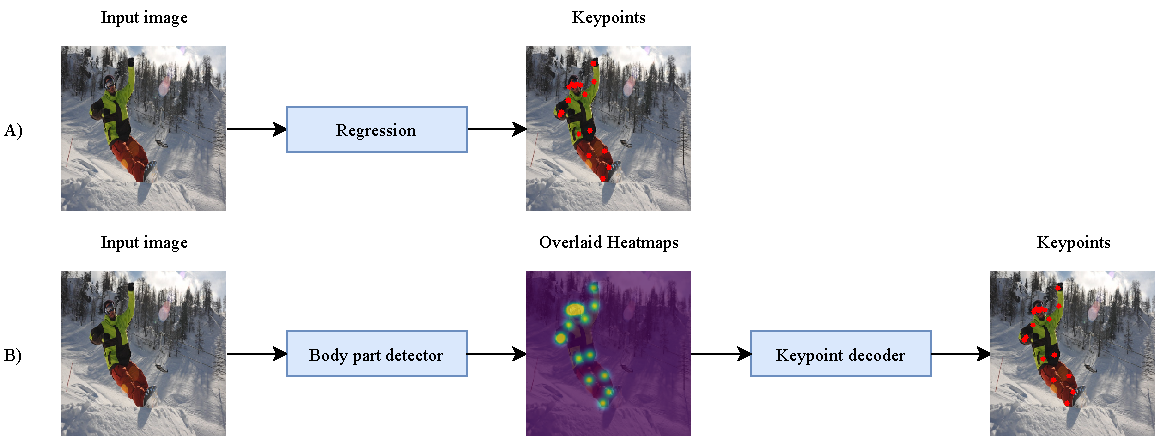
\includegraphics[width=\textwidth]{images/pose_detection.pdf}
    \caption{Regressions- und Körperteildetektions-Verfahren
    zum Bestimmen von Schlüsselpunkten eines Menschen. A) Ein Regressor
    versucht direkt die Punkte des menschlichen Körpers als Koordinaten
    auszugeben. B) Ein Körperteildetektor erzeugt eine Wärmekarte für jeden
    Schlüsselpunkt. Die Werte in den Karten geben die Wahrscheinlichkeit für den
    Aufenthalt eines Punktes an. Die Schlüsselpunkte müssen nach der Detektion aus den Karten dekodiert werden.}
    \label{fig:pose-detection}
\end{figure}

Ein Forschungsteam von Google hat ein neues Machine-Learning-Modell namens
\textit{MoveNet} \cite{movenet} präsentiert, das unter anderem auf mobilen
Geräten ausgeführt werden kann und dabei eine Echtzeiterkennung von menschlichen
Posen ermöglicht. Die Architektur besteht aus einem MobileNetV2-Backbone mit
angehängtem Feature-Pyramid-Network (FPN) und insgesamt vier Prediction-Heads,
die CenterNets \cite{zhou2019objects} sind. Trainiert wurde das Netzwerk
auf den COCO-Datensatz und erreicht laut den Autoren 30 oder mehr FPS auf
modernen Computern, Laptops und Smartphones. Auch dieses Modell verwendet
Wärmekarten, um mögliche Positionen von menschlichen Schlüsselpunkten zu
bestimmen und wird von einem Prediction-Head übernommen. Ein weiterer ist dafür
zuständig, den Abstand (Offset) jedes Pixels als Vektor von der geschätzten
Schlüsselpunktposition zu bestimmen. Ein anderer Kopf übernimmt die Gruppierung
der Schlüsselpunkte und ordnet diesen Personeninstanzen zu. Der vierte Kopf
schätzt das Zentrum der Instanzen. Die vollständige Architektur von MoveNet ist
in Abbildung \ref{fig:movenet-architecture} zu sehen.

\begin{figure}
    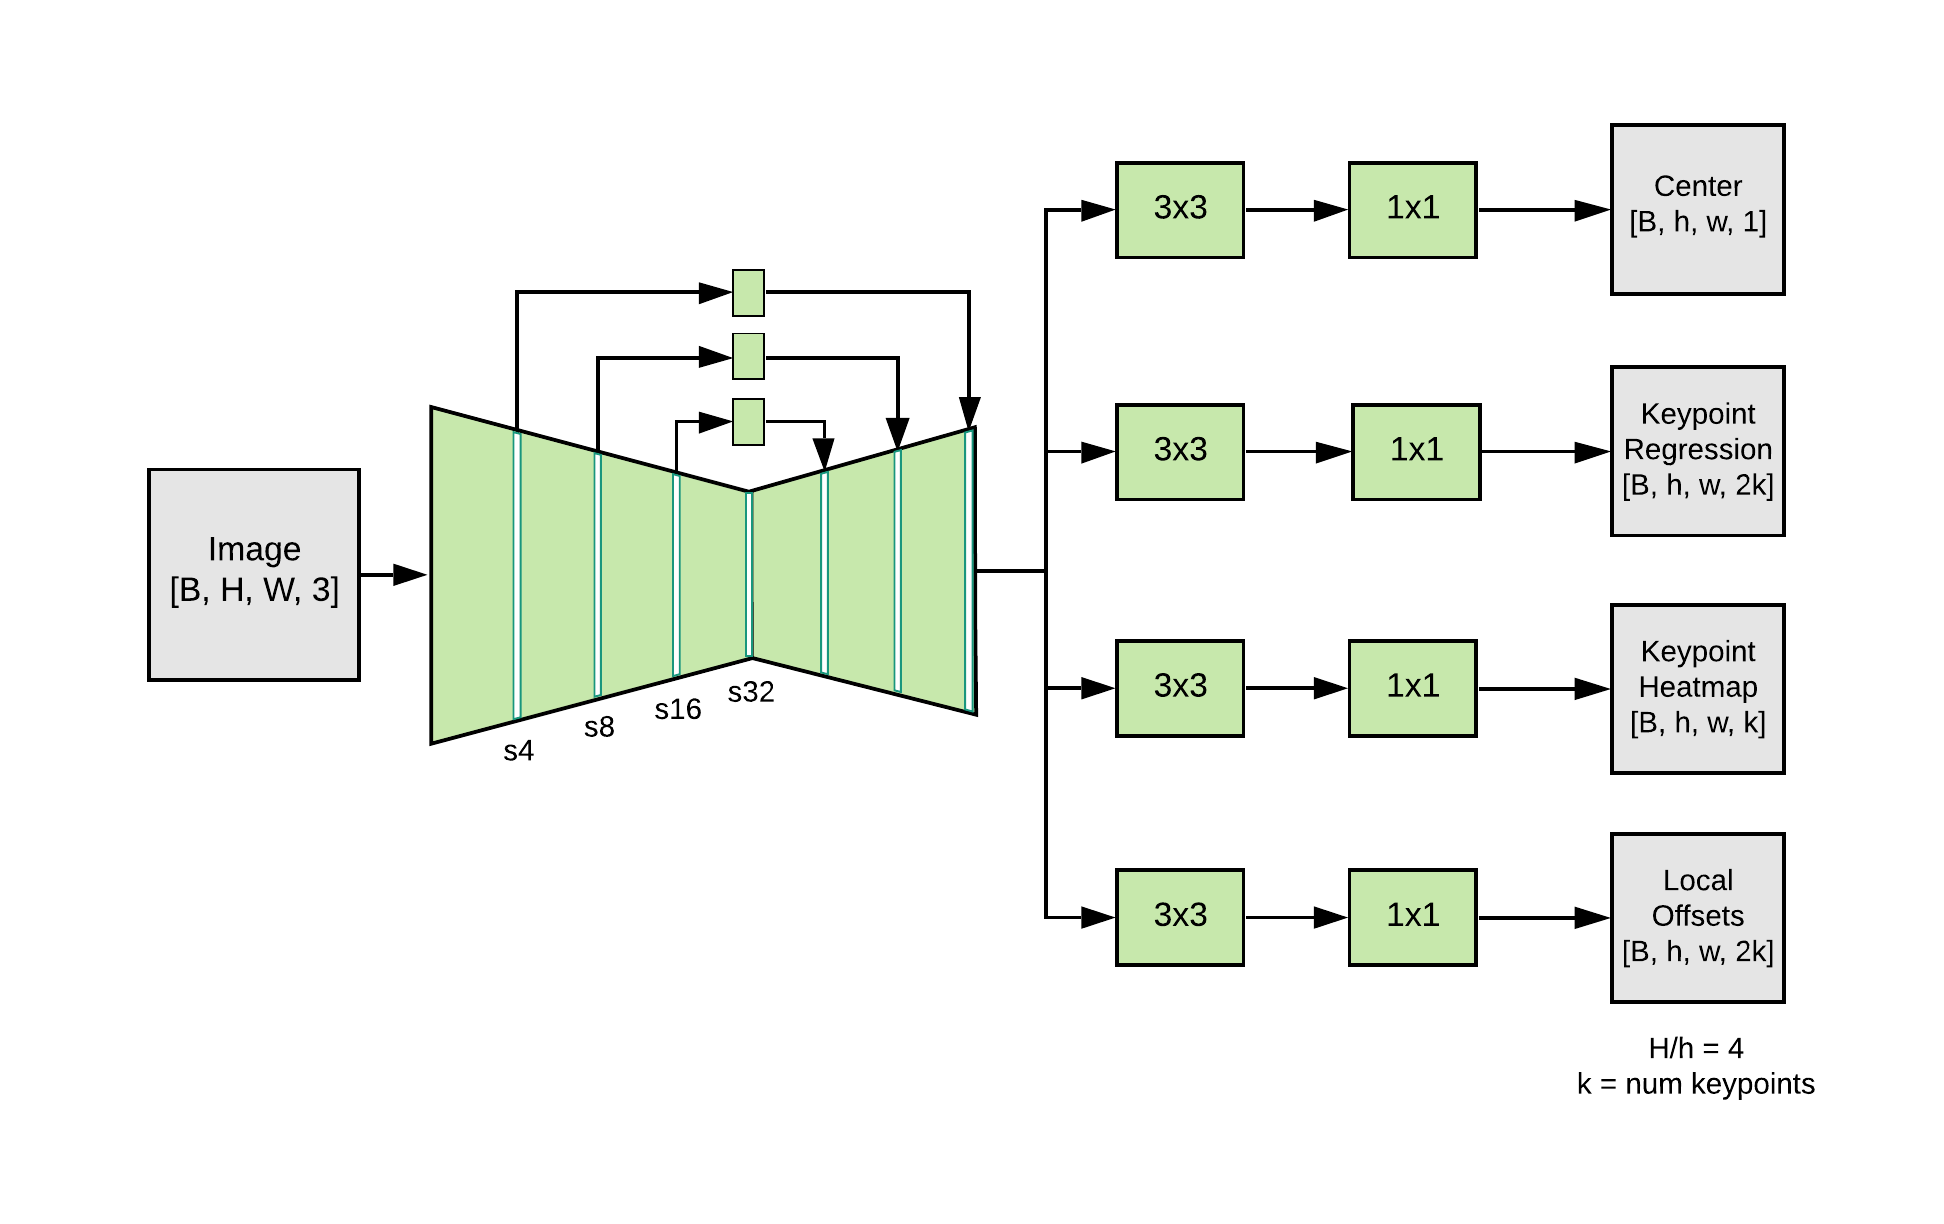
\includegraphics[width=\textwidth]{images/movenet_architecture.png}
    \caption{Architektur von MoveNet \cite{movenet}. Der Feature-Extractor
    besteht aus einem vortrainierten MobileNetV2-Backbone mit angehängtem FPN.
    Insgesamt werden vier Prediction-Heads zum Bestimmen von Schlüsselpunkten
    verwendet.}
    \label{fig:movenet-architecture}
\end{figure}

\section{Erkennung von Bewegungsarten}
Bei der Erkennung von Bewegungsarten handelt es sich um ein
Klassifizierungsproblem, bei der es darum handelt, eine Bewegungsaufzeichnung
einer Klasse zuzuordnen. Zu einer beliebigen Bewegungssequenz soll also eine
Aussage getroffen werden, ob es zum Beispiel Hantelübungen sind. Im Laufe dieses
Abschnitts soll dementsprechend ein Machine-Learning-Modell entworfen werden,
welches auf diese Aufgabe trainiert wird. Hierzu muss vorerst definiert werden,
welche Daten verwendet werden und wie diese für das Training vorbereitet werden
können. Damit eine Ortsänderung eines zu betrachtenden Objektes aufgezeichnet
werden kann, müssen mehrere Bilder bzw. Videos aufgezeichnet werden. Eine
Bewegung anhand eines einzelnen Bildes ist nicht möglich, da die Information
über die Ortsänderung dann nicht vorhanden ist. Es gilt also einen Datensatz zu
finden, welcher verschiedene Bewegungen im Videoformat bereitstellt. Alternativ
muss ein entsprechender Datensatz ausgehoben werden, was einen relativ hohen
Zeitaufwand bedeuten würde. Es wird aufgrund seiner Einfachheit der
UCF101-Datensatz \cite{ucf101} verwendet. Dieser besteht aus 101 Bewegungsarten
in Form von Videos, die öffentlich auf der Plattform YouTube zur Verfügung
stehen. Ein Videoclip ist dabei eindeutig einer Bewegungsklasse zugeordnet. Um
den Datensatz künstlich zu erweitern bzw. um eine Augmentation durchzuführen,
wird das KpGAN aus Kapitel \ref{chapter:gans} verwendet. Dieses erzeugt während des Trainings Schlüsselpunktdaten auf Nachfrage.

Es wird nun ein Modell entworfen, welches $n$ Frames eines Videos einliest und
die geschätzte Bewegungsklasse für diese Frames ausgibt. Dabei soll das Netzwerk
lernen, menschliche Posen aus den Frames zu extrahieren und anschließend zu
klassifizieren. Da das Neutrainieren der Posenerkennung zu lange dauern würde,
wird ein vortrainiertes MoveNet als Backbone verwendet. Für die Klassifizierung
werden verschiedene Köpfe implementiert, die anschließend miteinander verglichen
werden. Ziel ist es herauszufinden, welche Architekturen für den Gebrauch auf
mobilen Plattformen geeignet sind. Als Testplattform wird, wie einleitend beschrieben, Android verwendet.

Die zu betrachtenen Metriken sind Genauigkeit und
Aus\-führ\-ungs\-ge\-schwin\-dig\-keit. Als erstes werden einfache
Fully-Connected-Layer verwendet und evaluiert. Es wurden dabei Schritt für
Schritt Änderungen an der Anzahl der Neuronen und Schichten vorgenommen.
Anschließend wird untersucht, ob das Verwenden CNNs ähnliche oder bessere
Ergebnisse liefert, besonders in Hinblick auf die Performance. In Tabelle
\ref{table:motion-detection} sind die durchgeführten Experimente aufgelistet.

Das Ergebnis aus den Trainingsversuchen mit rein-realen Datensätzen ist, dass
CNNs die Bewegungen wesentlich besser erkennen können als die
Fully-Connected-Modelle. Nicht nur, dass sie hier eine höhere Genauigkeit
aufweisen, sie lernen die Verteilung auch wesentlich schneller. Während die
Fully-Connected-Modelle 300 Epochen für eine Genauigkeit von 90-97\% benötigen,
benötigen die CNNs lediglich 9-80 Epochen für bessere Resultate. Der einzige
Nachteil besteht in ihrer Ausführungsgeschwindigkeit, die bis zu vier mal
kleiner ist.

Erstaunlicherweise verhält sich dies bei den Trainingsversuchen mithilfe eines
GANs ein wenig anders. Grundsätzlich erreichten die Fully-Connected-Modelle eine
wesentlich höhere Genauigkeit nach sehr viel weniger Trainingsepochen. Die
Genauigkeit wurde dabei nicht mithilfe von synthetischen Daten des GANs
gemessen, sondern es wurden hierfür wieder echte Daten verwendet. Damit wurde
sichergestellt, dass die Genauigkeiten der verschiedenen Trainingsmethoden
vergleichbar gehalten werden. Das Verwenden von künstlich erzeugten Daten
liefert in diesem Fall also immer bessere Ergebnisse. Dies liegt vermutlich
unter anderem daran, dass GANs die Eigenschaft besitzen, zwischen echten Daten
zu interpolieren und damit automatisch eine Augmentation durchzuführen. Dies
führt dazu, dass die Modelle eine höhere Vielfalt lernen können. Diese Vielfalt
ist im echten Datensatz nicht so ausgeprägt. Hierbei ist wichtig zu erwähnen,
dass das Daten erzeugende GAN auf eben diesen Datensatz trainiert wurde. Der
Datensatz wurde also verbessert, indem ein GAN verwendet wurde, die Verteilung
zu lernen und zu interpolieren, um eine größere Datenvielfalt zu erzeugen.

\begin{table}
    \footnotesize
    \begin{tabularx}{\textwidth}{l|X|c|c|c|c|c}
        \hline
        name & layers & epochs & $p_\mathrm{real}$ & epochs & $p_\mathrm{gan}$ & inference speed \\ \hline

        \multirow{3}{*}{linear} & Dense, 128 \newline ReLU \newline Dense, 3 & 300 & 0.90 & 82 & 0.99 & \num{0.59e-6}s \\ \cline{2-7}

        & Dense, 256 \newline ReLU \newline Dense, 3 & 300 & 0.94 & 49 & 0.99 & \num{0.61e-6}s \\ \cline{2-7}

        & Dense, 128 \newline ReLU \newline Dense, 256 \newline ReLU \newline Dense, 3 & 300 & 0.97 & 70 & 0.99 & \num{0.83e-6}s \\ \hline

        \multirow{3}{*}{conv} & Conv2D, 16, $3 \plh 3$, stride 2 \newline Conv2D, 32, $3 \plh 3$, stride 2 \newline Dense, 3 & 81 & 0.99 & 123 & 0.99 & \num{1.25e-6}s \\ \cline{2-7}

        & Conv2D, 16, $3 \plh 3$, stride 2 \newline Conv2D, 32, $3 \plh 3$, stride 2 \newline Conv2D, 64, $3 \plh 3$, stride 2 \newline Dense, 3 & 44 & 0.99 & 121 & 0.99 & \num{1.74e-6}s \\ \cline{2-7}

        & Conv2D, 16, $3 \plh 3$, stride 2 \newline Conv2D, 32, $3 \plh 3$, stride 2 \newline Conv2D, 64, $3 \plh 3$, stride 2 \newline Conv2D, 128, $3 \plh 3$, stride 2 \newline Dense, 3 & 9 & 0.99 & 126 & 0.99 & \num{2.27e-6}s \\ \hline
    \end{tabularx}
    \caption{Durgeführte Experimente mit verschiedenen Architekturen für die
    Bewegungserkennung. Die Eingabe besteht aus 60 Frames einer
    Bewegungsanimation aus 17 Schlüsselpunkten mit jeweils 3 Eigenschaften (x-,
    y-Koordinaten und Wahrscheinlichkeitsscore) kodiert als Bild (siehe
    Abbildung \ref{fig:motion-images}). Als Ausgabe sollen die Netze die
    geschätzte Klasse, also das Label liefern. $p_\mathrm{real}$ gibt die
    Genauigkeit des jeweiligen Modells an, das mit einem realen Datensatz
    trainiert wurde. $p_\mathrm{gan}$ gibt hingegen die Genauigkeit der Modelle
    an, die mithilfe eines KpGAN-Generators trainiert wurden. Für das Messen der
    Genauigkeit wurden immer reale Daten verwendet.}
    \label{table:motion-detection}
\end{table}